\section{Design}

\subsection{High Level Overview}

The system will comprise 3 parts required to simulate and program a proprietary processor. It will include a virtual machine to emulate the execution of binary machine code catridges, an assembler to translate higher level assembly code into machine code, and finally a compiler for a higher level language to easily program complex applications to run on the processor.

The virtual machine consists of two main processes, the debugger and interpreter. The interpreter will continiously step through memory, decoding and executing instructions sequentially whilst displaying the contents of VRAM through the pixel display.

\bigskip

\shadowbox{
    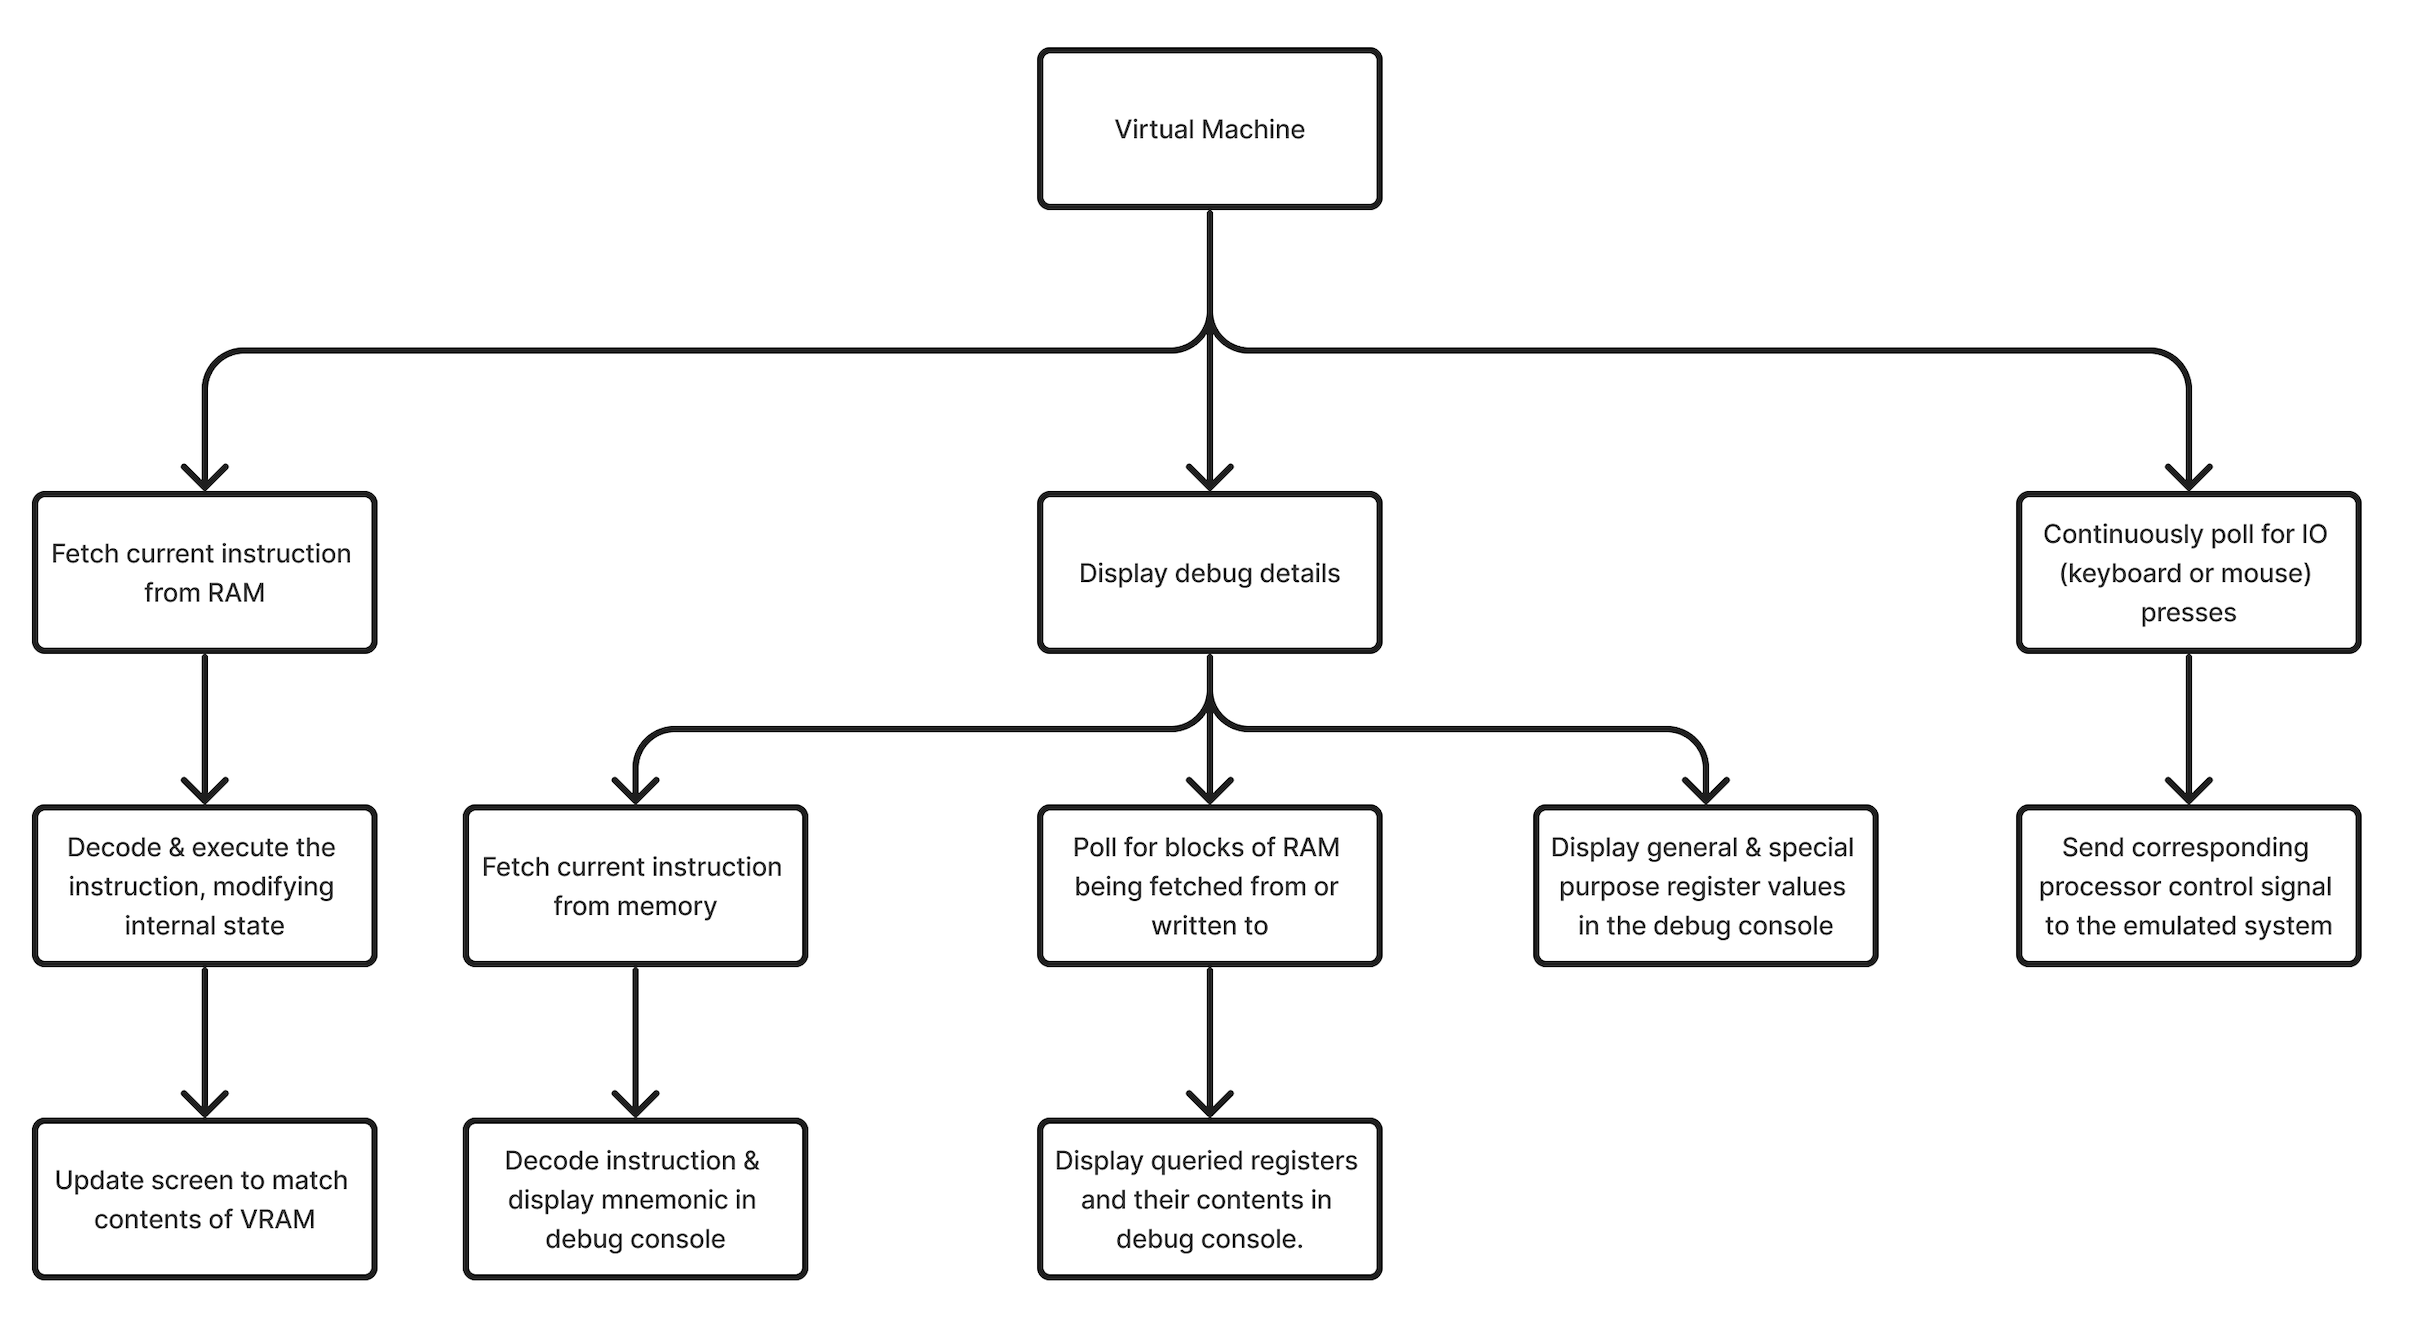
\includegraphics[width=13cm]{Screenshot 2024-07-23 at 13.51.25.png}
}

\bigskip

\begin{multicols}{2}[\columnsep-0.5em] 
    The assembler consists of a single pipeline for transforming ASCII assembly programs into binary machine code. The files are loaded into the interpreter which stores their contents in a string. The contents are then tokenised by a lexer into a list of objects representing the foundational elements of the program (e.g. STRING, BRACE, NUMBER) and parsed into a sequence of assembly language instructions. These instructions are translated into binary machine code according to the instruction set architecture (defined in \ref{sec:MachineCodeEncoding}) which is then written to a file and stored on the users computer.


    \columnbreak

    \shadowbox{
        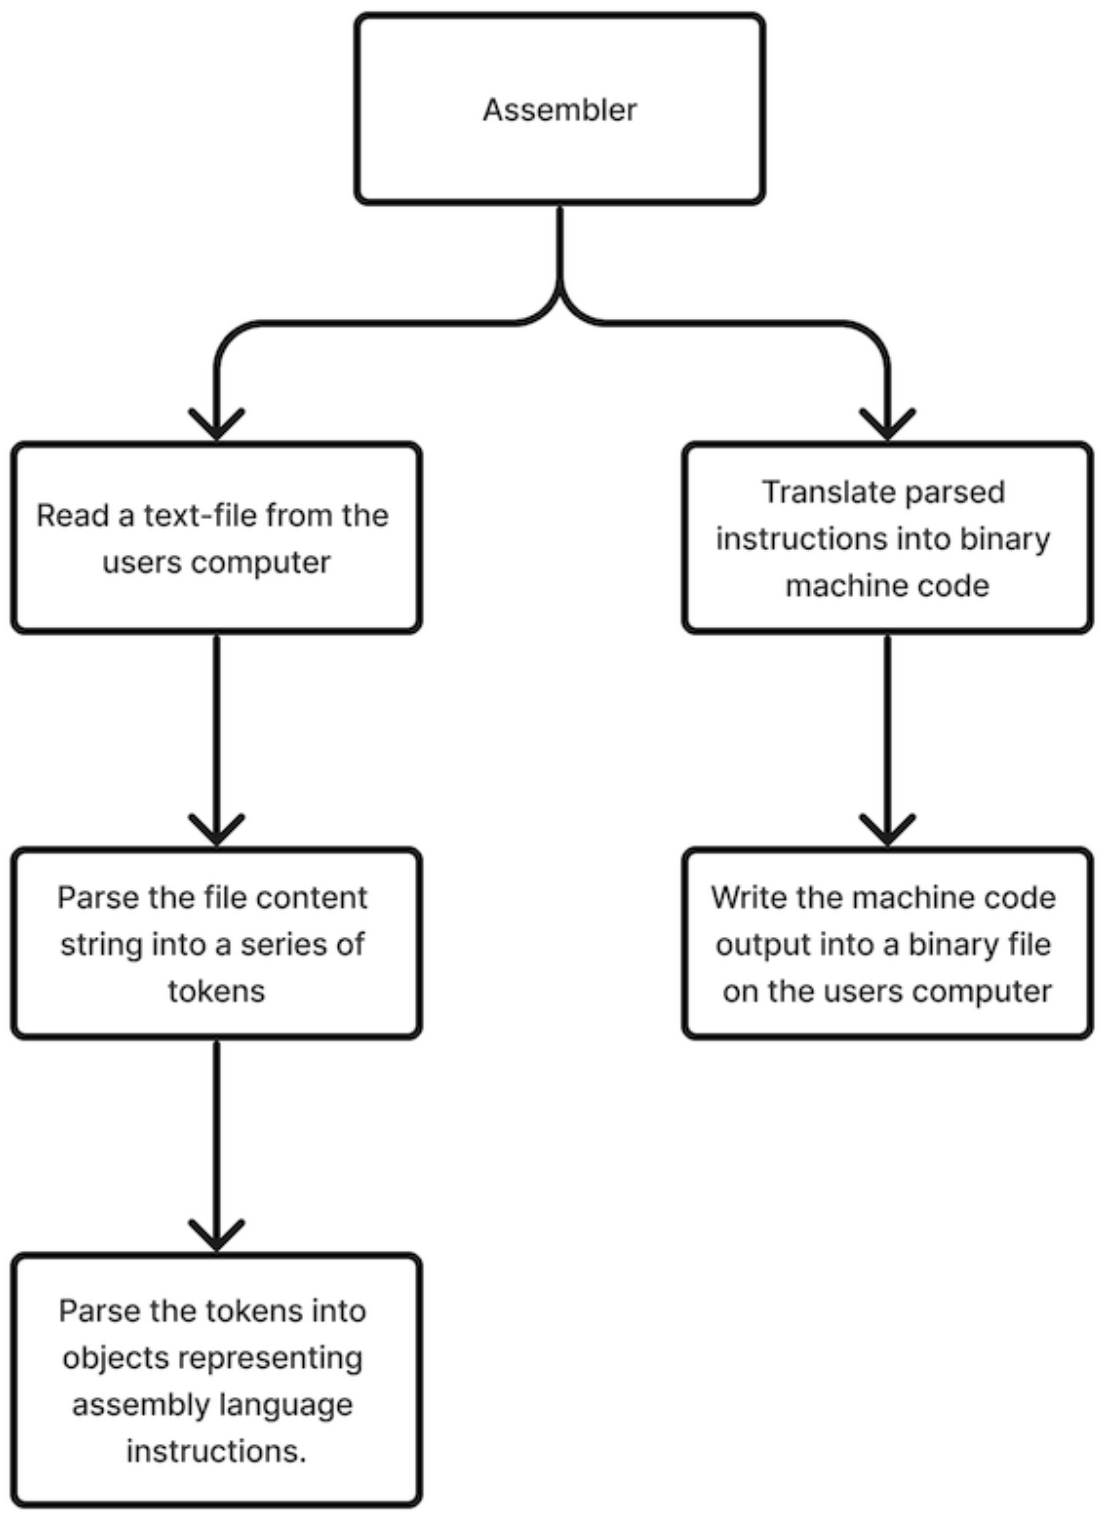
\includegraphics[width=5cm]{Screenshot 2024-07-23 at 12.47.14.png}
    }

\end{multicols}


\begin{wrapfigure}[13]{r}{8.5cm}
\shadowbox{
    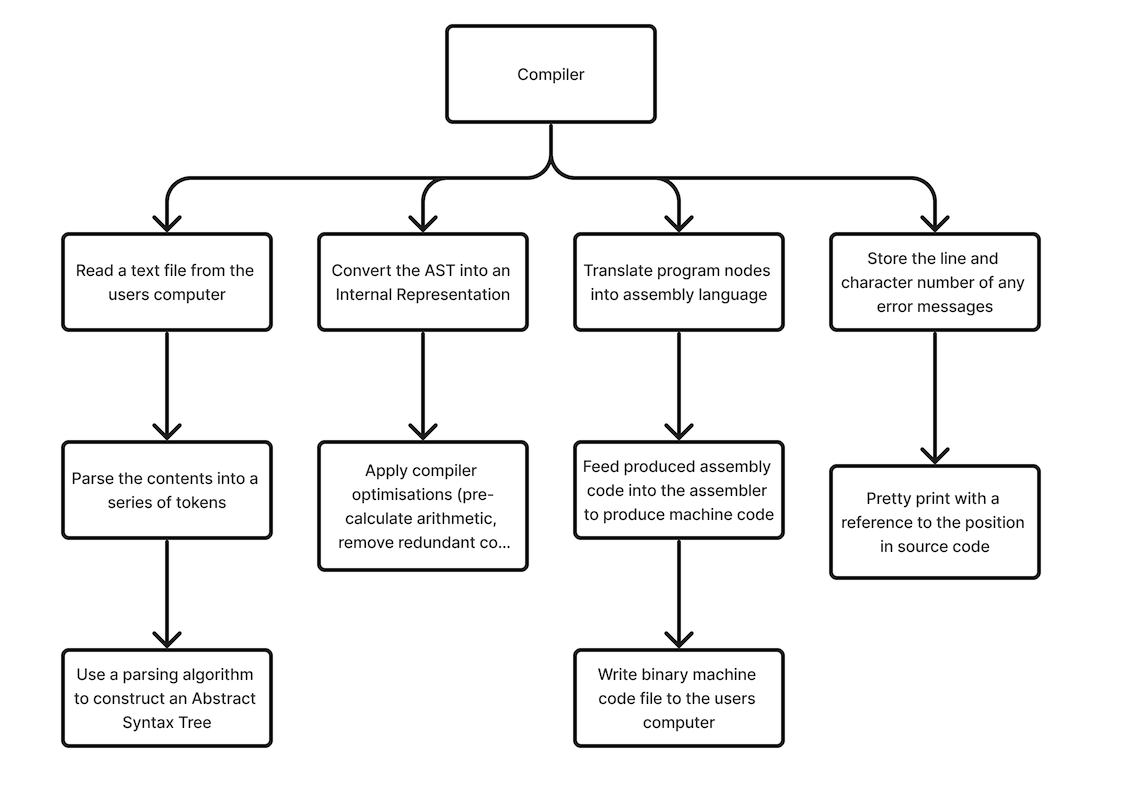
\includegraphics[width=8cm]{Screenshot 2024-06-24 at 19.30.50.png}
}
\end{wrapfigure}

\begin{samepage}

Much like the assembler, the compiler takes an ASCII program, converts it into tokens and parses it into an Abstract Syntax Tree (AST) representing the structure and order of operations of the program. This AST is converted into an internal representation (IR) designed to help easily locate potential optimisations in the source code (e.g. pre-calculating arithmetic or removing redundant code), these optimisations are made and the IR is converted into an intermediate assembly language due to the presence of high level optimisations such as labels and macro-instructions. Finally, this assembly code is inserted into the assembler and the produced machine code is stored as a file on the users computer. 

\end{samepage}

\bigskip

\subsection{Component Design}
\subsubsection{Instruction Set Architecture}

\subsubsubsection{Computer Architecture}
Having to balance simplicity with convenience dictated the final design decisions for this computers CPU architecture.  There is 64Kb of memory (65,526 memory locations) specified by 16-bit addresses, requiring a 16-bit Program Counter (PC). The clock speed for the CPU runs at 600Hz. Each instruction is 32-bits, meaning two processor cycles are required to fetch an instruction and store the high and low words in the Current Instruction Register (CIR). 

I decided on 32 16-bit general purpose registers, any two of which can be inputs to the ALU, which itself has two outputs - a 16 bit result which can be written to a register or memory depending on the instruction, and a 1 bit zero bit which is set when the result of the calculation is 0.

There are a number of special purpose registers, which, by convention are dedicated an address in memory, one for the stack pointer (SP) and another for the sound timer (ST). There is no dedicated stack and is instead allocated a downwards growing section of memory. The stack stores register values and return addresses when calling functions, however since the instruction set contains no \texttt{call} or \texttt{ret} instructions, this must be performed manually by the programmer. Each cycle the sound timer is non-zero, the computer produces a sound and decrements ST, allowing the length of the noise to be specified.

\needspace{100pt}

\subsubsubsection{Arithmetic and Logic Unit}

\begin{wrapfigure}[10]{r}{6.5cm}
    \shadowbox{
        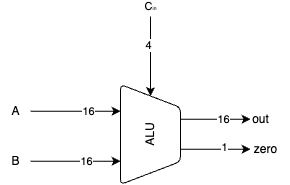
\includegraphics[width=6cm]{ALU schema.png}
    }
\end{wrapfigure}

The core of any instruction set is the Arithmetic Logic Unit (ALU) so I began by designing an interface for that. I decided on 2 16-bit inputs to the ALU, which can either take register values, or for an Ri-type instruction, the value of the 16-bit immediate field. There are 4 ALU control bits into the ALU, whcih dictate the operation to be performed. The first two control bits negate their respective inputs, and the second two determine the arithmetic or logical operation to perform. Combinations of these ALU control bits can produce a variety of different operations, all of which are detailed in the table below. (\cite{EOCS})

\bigskip

\begin{center}
    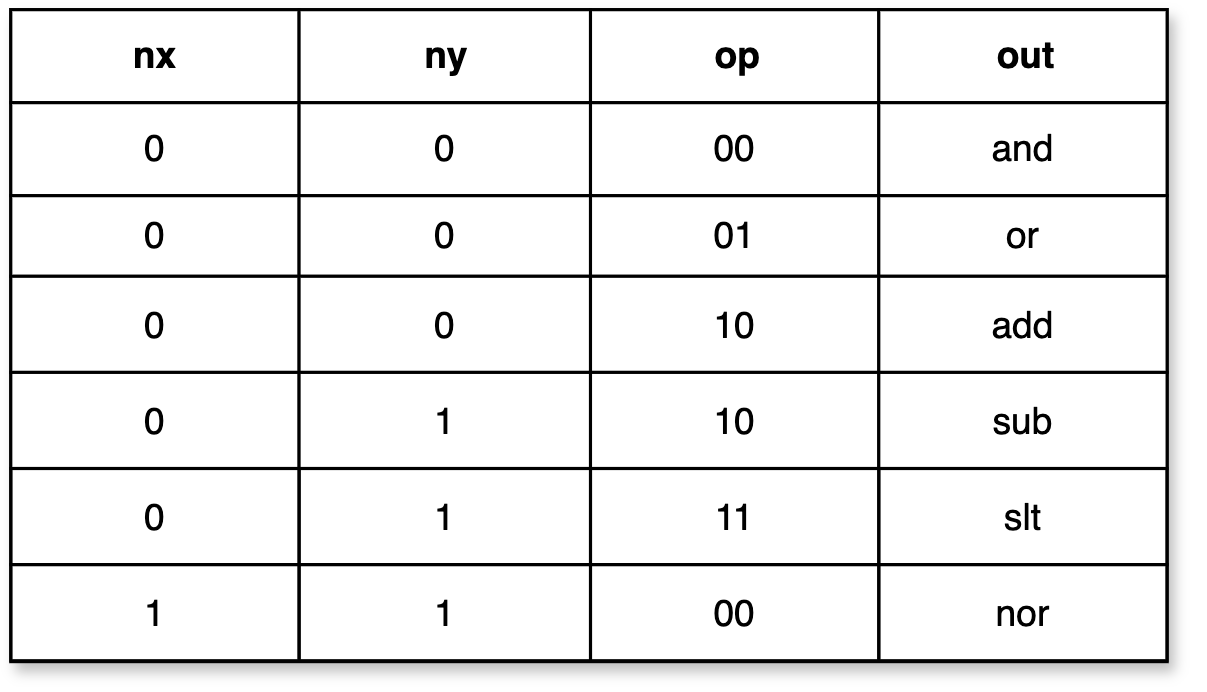
\includegraphics[width=8cm]{Screenshot 2024-08-29 at 19.34.16.png}
\end{center}

\subsubsubsection{Assembly Language}

I decided to use a MIPS instruction set architecture, minimising the number of instructions supported by the processor. I settled on 3 instruction types: R-type instructions (performing ALU operations on register values), I-type instructions (operations involving both registers and immediate fields), and J-type instructions (unconditional, absolute jumps to locations in memory). From these 3 types, the following instruction set can be constructed, demonstrated with a program to multiple two numbers stored in memory. (\texttt{'[]'} are used to indicate a memory address):

\begin{lstlisting}[language=C]
R-type: add, sub, and, or, nor, slt, sll, slr
I-type: addi, andi, ori, lw, sw, bge, bne
J-type: jmp

// multiply the numbers in memory address 0xb000 and 0xb001, and write the answer to 0xb002
li r31, 0xb000 // pointer to the start of data memory

lw r1, 0($r31)
lw r2, 1($r31)

.loop
    // if r2 is 0, break
    li r0, 0
    beq r0, r2, [.store]

    add r1, r1, r1

    addi r2, r2, -1

    jmp [.loop]

.store
    sw r1, 2($r31)
\end{lstlisting}

\subsubsubsection{Machine Code Encoding}
\label{sec:MachineCodeEncoding}

Below is the breakdown of how R/I/J type instructions are represented in binary, broken down into their respective fields. All instructions have a 4-bit opcode which dictates the type of instruction (and consequentially which of 4 encoding types should be used when decoding the instruction). For the purpose of machine code, L and Ri type instructions are encoded with the same fields.

\begin{itemize}
    \item \texttt{00-xx}: R-type instructions \textit{to perform operations between two registers}
        \begin{itemize}
            \item \texttt{5-bits rs}: the first of two input registers to the ALU.
            \item \texttt{5-bits rt}: the second of two input registers to the ALU.
            \item \texttt{5-bits rd}: the register in  which to store the result of the operation.
            \item \texttt{4-bits func}: the control bits determining the ALU operation.
        \end{itemize}
    \item \texttt{01-xx}: Ri-type instructions \textit{(to perform operations between a register and immediate value)}
        \begin{itemize}
            \item \texttt{5-bits rs}: the first of two input registers to the ALU.
            \item \texttt{5-bits rt}: the second of two input registers to the ALU.
            \item \texttt{16-bits immediate}: the data used as the second ALU input.
        \end{itemize}
    \item \texttt{10-xx}: L-type instructions \textit{(to load/store words from memory)}
        \begin{itemize}
            \item \texttt{5-bits rs}: the register containing the base offset for calculating memory addresses.
            \item \texttt{5-bits rt}: the register to store/read data from/into memory.
            \item \texttt{16-bits immediate}: the offset from the base address for the calculating memory addresses.
        \end{itemize}
    \item \texttt{11-xx}: J-type instructions \textit{(to unconditionally jump an absolute location in memory)}
        \begin{itemize}
            \item \texttt{16-bits address}: the memory address to jump to.
        \end{itemize}
\end{itemize}
 
\bigskip

\begin{center}
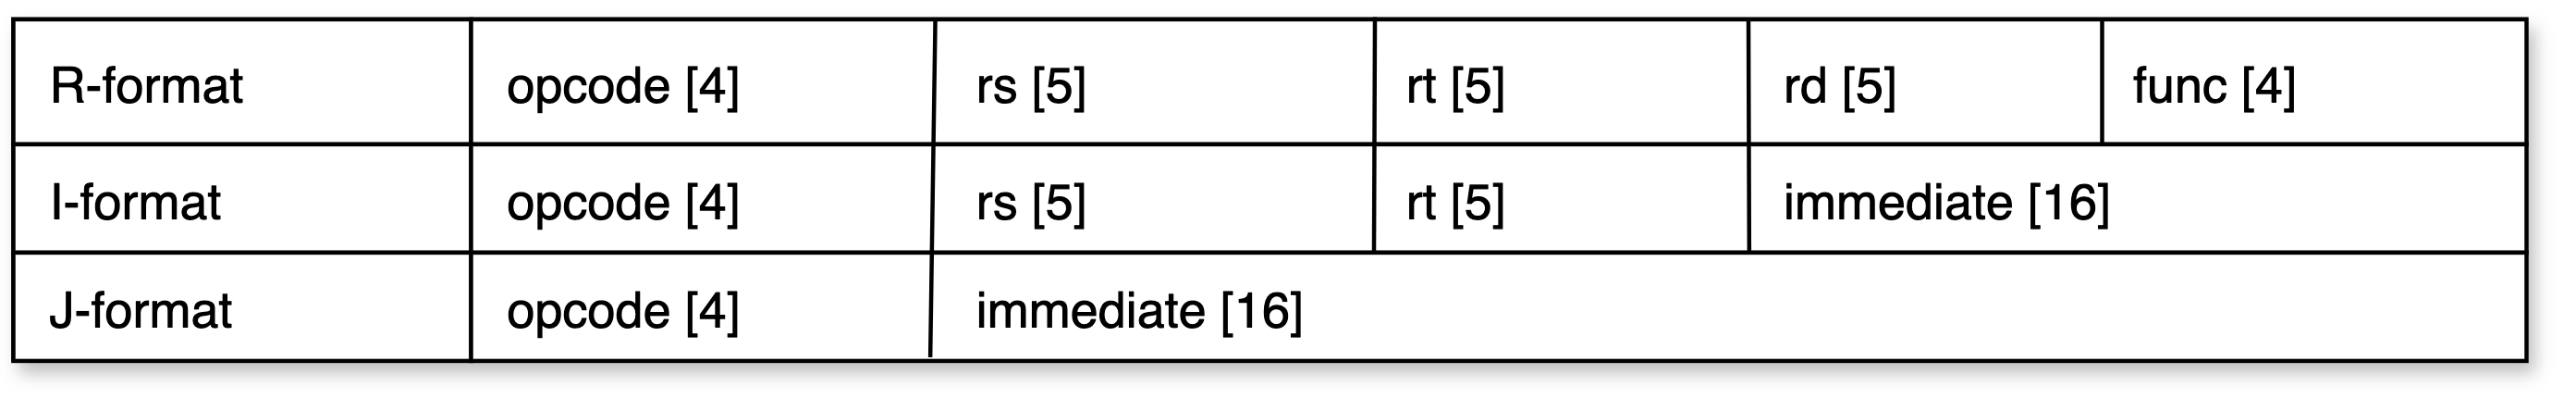
\includegraphics[width=14cm]{Screenshot 2024-08-29 at 22.34.18.png}
\end{center}

\bigskip

Next to each assembly instruction below is its machine code encoding, showing the relationship between the assembly language operands and the encoding fields. 

\begin{lstlisting}
addi $r5, $r0, 14      // 0110 00000 00101 00000000 00001110
lw $r4, 10($r30)       // 1000 11110 00100 00000000 00001010


slt $r0, $r1, $r2z     // 0000 00001 00010 00000 0111 
bne $r0, $r4, [0xb020] // 1101 00000 00100 10110000 00100000
jmp [0x8080]           // 1111 10000000 10000000
\end{lstlisting}

\subsection{Virtual Machine}
\subsubsection{Data Structures}
\subsubsection{Algorithms}